\documentclass[a4paper]{scrartcl}

\usepackage[english,nswissgerman]{babel} % language settings
\usepackage[utf8]{inputenc} % input encoding for äöü
\usepackage{amsmath} % math
\usepackage[T1]{fontenc} % fonts better printed
\usepackage{amssymb} % math
\usepackage{siunitx} % SI units
\usepackage{tikz} % graphics
\usepackage{circuitikz} % electronic circuits
\usepackage{color} % colors
\usepackage{graphicx} % include graphics
\usepackage{listings} % sourcecode
\usepackage{enumitem} % enumerations
\usepackage{wrapfig} % figures around text
\usepackage{booktabs} % tables
\usepackage{pgfplotstable} % tables form csv
\usepackage{hyperref}



% si setup
\sisetup{
	round-mode=places,
	round-precision=2
}

\begin{document}
	\tableofcontents
	\newpage
	\section{some math}
		$\int_{a}^{b} f(x) \,\mathsf{d}x=F(b)-F(a)$
		
		\begin{align}
			0&=(x-1)^2(x-2)(x+1) \\
			(x+1)&=(x-1)^2(x-2) 
		\end{align}
		
		\num{1} \si{kg.m/s^2}\\
		
		\SI[per-mode=fraction]{1.3445}{\meter\per\second}
		
	\section{images}
		\begin{figure}[hb]
			\centering
			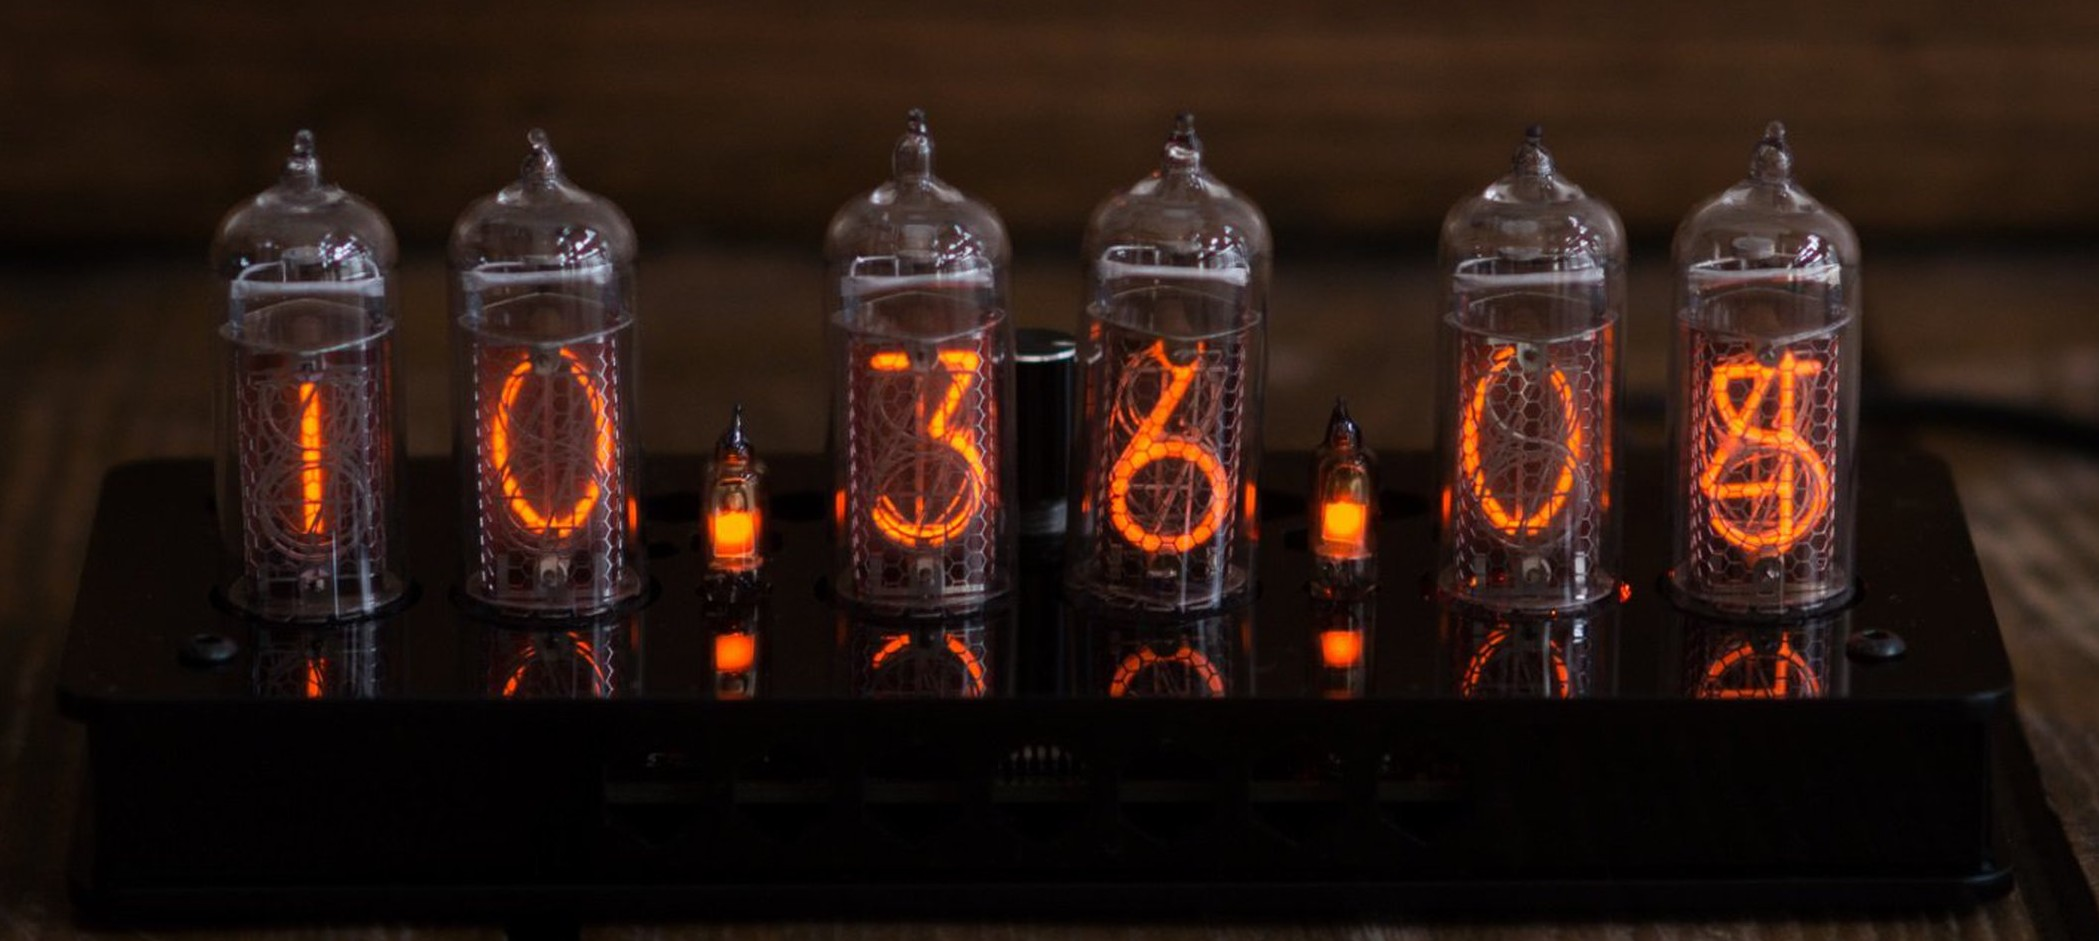
\includegraphics[width=\textwidth]{img/nixie.jpg}
			\caption{Nixie!!}
			\label{fig:nixie}
		\end{figure}
	
		Pic \ref{fig:nixie}
	
		\begin{wrapfigure}[]{l}[0pt]{5.1cm}
			\centering
			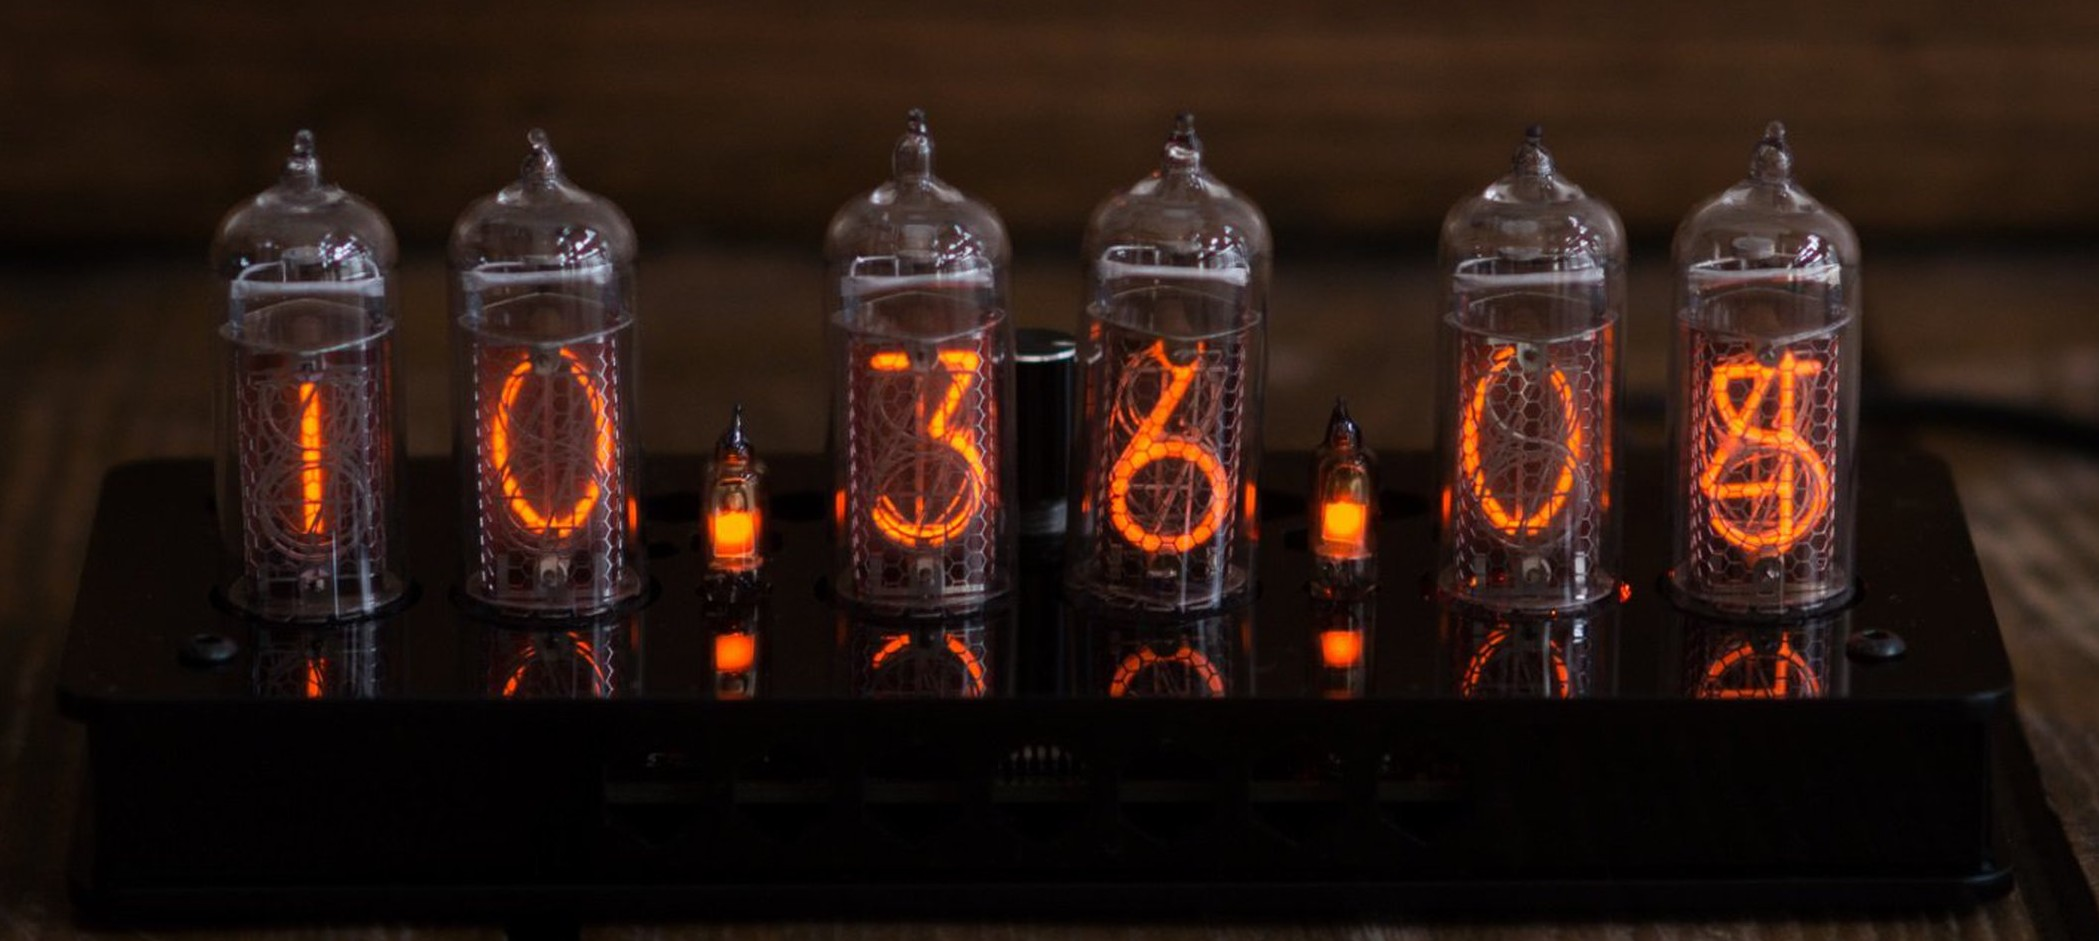
\includegraphics[width=5cm]{img/nixie.jpg}
			\caption{Nixie!!}
			\label{fig:nixie2}		
		\end{wrapfigure}
	
		Dies hier ist ein Blindtext zum Testen von Textausgaben. Wer diesen Text liest, ist selbst schuld. Der
		Text gibt lediglich den Grauwert der Schrift an. Ist das wirklich so? Ist es gleichgültig, ob ich schreibe:
		„Dies ist ein Blindtext“ oder „Huardest gefburn“? Kjift – mitnichten! Ein Blindtext bietet mir wichtige In-
		formationen. 		Dies hier ist ein Blindtext zum Testen von Textausgaben. Wer diesen Text liest, ist selbst schuld. Der
		Text gibt lediglich den Grauwert der Schrift an. Ist das wirklich so? Ist es gleichgültig, ob ich schreibe:
		„Dies ist ein Blindtext“ oder „Huardest gefburn“? Kjift – mitnichten! Eine Blindtext bietet mir wichtige Informationen.
		

	\newpage
		
	\section{enumerates}
		\begin{enumerate}[noitemsep]
			\item first
			\item second
			\begin{enumerate}
				\item erstes
				\item zweites
				\begin{enumerate}
					\item AA
					\item BB
					\begin{enumerate}
						\item aa
						\item bb
						\begin{itemize}
							\item[first] blah
						\end{itemize}
					\end{enumerate}
				\end{enumerate}
			\end{enumerate}
		\end{enumerate}
		\begin{itemize}
			\item A
			\begin{itemize}
				\item B 
				\begin{itemize}
					\item C 
					\begin{itemize}
						\item D 
					\end{itemize}
				\end{itemize}
			\end{itemize}			
		\end{itemize}
	
	\section{TikZ}
		\subsection{a}
			\begin{tikzpicture}
				\draw (0,0) rectangle (1,2);
				\draw [->](2,1) -- (3,1);
				\draw (5,1) circle (1);
			\end{tikzpicture}
			
		\subsection{b}
			\begin{tikzpicture}
				\draw[red] (2,2) circle (0.5);				
				\draw[yellow] (2,2) circle (1);
				\draw[green] (2,2) circle (1.5);
			\end{tikzpicture}
	
		\subsection{c}
			\begin{tikzpicture}
				\draw[color=green,fill=red] (0,0) rectangle (2,1);
			\end{tikzpicture}

		\subsection{d}
			\begin{tikzpicture}
				\draw[->] (0,0) -- (3.2,0) node[right] {$x$};
				\draw[->] (0,-1) -- (0,1.2) node[above] {$y$};
				\draw plot[domain=0:3,smooth] (\x, { cos(\x r) } );
			\end{tikzpicture}
			
		\subsection{e}
			\begin{circuitikz}[european]
				\draw (0,2)
				to[V,v=$U_0$] (0,0)
				to[short] (2,0)
				to[R] (3,0)
				to[short] (4,0)
				to[C] (4,2)
				to[short] (4,2)
				to[short] (3,2)
				to[L] (2,2)
				to[short] (0,2)
				;
			\end{circuitikz}
	
	\section{Blindtext}
		Dies hier ist ein Blindtext zum Testen von Textausgaben. Wer diesen Text liest, ist selbst schuld. Der
		Text gibt lediglich den Grauwert der Schrift an. Ist das wirklich so? Ist es gleichgültig, ob ich schreibe:
		„Dies ist ein Blindtext“ oder „Huardest gefburn“? Kjift – mitnichten! Ein Blindtext bietet mir wichtige In-
		formationen.
		
		\subsection{Unterabschnitt}
			Dies hier ist ein Blindtext zum Testen von Textausgaben. Wer diesen Text liest, ist selbst schuld. Der
			Text gibt lediglich den Grauwert der Schrift an. Ist das wirklich so? Ist es gleichgültig, ob ich schreibe:
			„Dies ist ein Blindtext“ oder „Huardest gefburn“? Kjift – mitnichten! Ein Blindtext bietet mir wichtige In-
		
			\subsubsection{Eine Ebene tiefer}
				Dies hier ist ein Blindtext zum Testen von Textausgaben. Wer diesen Text liest, ist selbst schuld. Der
				Text gibt lediglich den Grauwert der Schrift an. Ist das wirklich so? Ist es gleichgültig, ob ich schreibe:
				„Dies ist ein Blindtext“ oder „Huardest gefburn“? Kjift – mitnichten! Ein Blindtext bietet mir wichtige
		
		\subsection{Weiterer Unterabschnitt}
			Dies hier ist ein Blindtext zum Testen von Textausgaben. Wer diesen Text liest, ist selbst schuld. Der
			Text gibt lediglich den Grauwert der Schrift an. Ist das wirklich so? Ist es gleichgültig, ob ich schreibe:
			„Dies ist ein Blindtext“ oder „Huardest gefburn“? Kjift – mitnichten! Ein Blindtext bietet mir wichtige In-
			formationen. An ihm messe ich die Lesbarkeit einer Schrift, ihre Anmutung, wie harmonisch die Figuren
			zueinander s
			
	\section{Wieder ganz oben in der Strukturhierarchie}
		Dies hier ist ein Blindtext zum Testen von Textausgaben. Wer diesen Text liest, ist selbst schuld. Der
		Text gibt lediglich den Grauwert der Schrift an. Ist das wirklich so? Ist es gleichgültig, ob ich schreibe:
	
\end{document}